\documentclass[12pt]{article}
\usepackage{amsmath}
\usepackage{graphicx}
\usepackage{hyperref}
\usepackage{xcolor}
\usepackage{subcaption}
\usepackage{siunitx}

\addtolength{\oddsidemargin}{-.875in}
\addtolength{\evensidemargin}{-.875in}
\addtolength{\textwidth}{1.75in}

\addtolength{\topmargin}{-.875in}
\addtolength{\textheight}{1.75in}

\title{Model Predictive Control}
\date{2020}
\author{sentry5588}

\begin{document}
\pagecolor{lightgray}
\maketitle
\section{Introduction}
This note documents the Model Predictive Control (MPC) method for the two
wheel balancing robot. Many people has built similar self-balancing robots.
Almost all of them uses PID control as the control strategy. For position
estimation, some uses Kalman filters, and others uses complementary filters.

The purpose of using MPC in this robot is not trying to invent a new MPC
technique, which usually the case for research papers.
But rather I intend to 1) practice MPC and 2) test how well MPC behaves
compares to other control schemes.

\section{Robot Coordinates}
As shown in Figure~\ref{fig_coordinates}, $\theta_k$ and $\omega_k$ denotes 
the angular position at time step $k$, respectively.
Counter-clockwise rotation is positive. Angular acceleration is denoted
by $\dot{\omega}_k$.
$u_k$ is the horizontal force
with positive to the right. Robot specifications can be found in 
Table~\ref{tab_robot_specification}


\begin{figure}

\begin{subfigure}{0.3\textwidth}
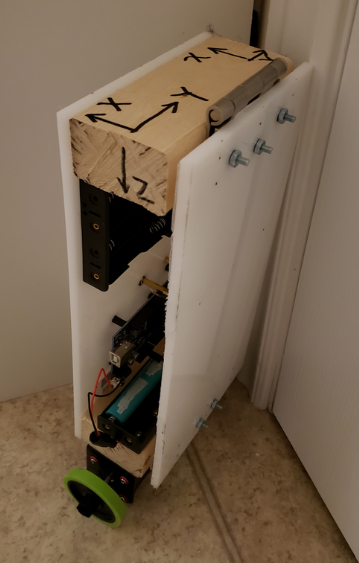
\includegraphics[width=\linewidth]{./figures/coordinates.png}
\caption{Robot Coordinates} \label{fig_coordinates}
\end{subfigure}
\hspace*{\fill} % separation between the subfigures
\begin{subfigure}{0.3\textwidth}
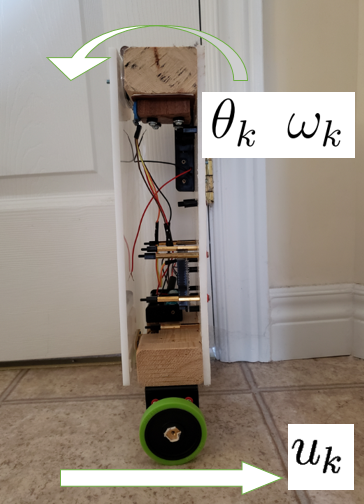
\includegraphics[width=\linewidth]{./figures/one_d_rotation.png}
\caption{1D Rotation} \label{fig_one_d_rotation}
\end{subfigure}
\hspace*{\fill} % separation between the subfigures
\begin{subfigure}{0.3\textwidth}
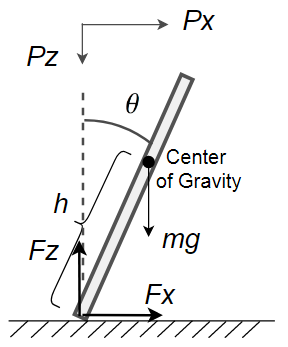
\includegraphics[width=\linewidth]{./figures/free_body_diagram.png}
\caption{1D Free Dody Diagram} \label{fig_1d_free_body_diagram}
\end{subfigure}
\caption{Two Wheel Balancing Robot} \label{fig_robots}
\end{figure}


\begin{table}
  \centering
  \begin{tabular}{l|c|c}
    \hline
	Specification & Notation & Value \\ \hline
    Center of Gravity (CoG) & $h$ & ?? 0.2 m \\ 
	Mass & $m$ & ?? 1.1 kg \\ 
	Moment of Inertia & I & ?? 0.8 \si{\kilogram\cdot\meter^2} \\ \hline
  \end{tabular}
  \caption{Robot specification} 
  \label{tab_robot_specification}
\end{table}


\section{Problem Formulation}
The model is a 1-input-2-output model.
\begin{align}
\label{equ_orig_nonlinear_dynamics}
x_{k+1} & = f(x_k, u_k) \\
y_k & = C(x_k)x_k
\end{align}

$x_k=[\theta_k\;\;\omega_k\;\;\dot{\omega}_k]^T$ is the system state. 
Linearize Equ~\ref{equ_orig_nonlinear_dynamics}, we have
\begin{align}
x_{k+1} & = A(x_k)x_k + B(x_k)u_k \\
y_k & = C(x_k)x_k
\end{align}

where $A(x_k)$ and $B(x_k)$ are Jacobians and given by
\begin{align}
A(x_k) = \frac{\partial f}{\partial x_k},
B(x_k) = \frac{\partial f}{\partial u_k}
\end{align}

Figure~\ref{fig_1d_free_body_diagram} is the 1-D free body diagram.
In the next subsection, I will develop the nonlinear continuous-time
dynamics.

\subsection{Nonlinear Continuous-Time Model}
Summing the forces in figure~\ref{fig_1d_free_body_diagram} in the horizontal
direction we have
\begin{align}
F_x=m\ddot{p}_x
\end{align}
where $p_x$ is the horizontal velocity of the CoG.
Summing the forces in figure~\ref{fig_1d_free_body_diagram} in the vertical
direction we have
\begin{align}
mg-F_z = m\ddot{p}_z
\label{equ_vertical_newton}
\end{align}
where $p_x$ is the horizontal velocity of the CoG.
Summing the torques in figure~\ref{fig_1d_free_body_diagram} around the
center of gravity we have
\begin{align}
F_x h\cos(\theta) + F_z h\sin(\theta) + mg\cdot 0= \ddot{\theta}I
\label{equ_rotation_newton}
\end{align}
\textcolor{blue}{
The contact point between the robot and the ground has $0$ vertical velocity.
It's vertical velocity is a combination of the rod rotation around 
CoG, $\dot{\theta}h\sin(\theta)$,
and vertical velocity of CoG, $\dot{p}_z$. Therefore
\begin{align}
-\dot{\theta}h\sin(\theta) + \dot{p}_z = 0
\label{equ_velocity_equation}
\end{align}
Take time derivative of~(\ref{equ_velocity_equation})
\begin{align}
-\ddot{\theta}h\sin(\theta) - \dot{\theta}^2h\cos(\theta) + \ddot{p}_z = 0\\
\ddot{p}_z = \ddot{\theta}h\sin(\theta) + \dot{\theta}^2h\cos(\theta)
\label{equ_ddot_p_z}
\end{align}}
Substitute $\ddot{p}_z$ in~(\ref{equ_vertical_newton}) 
with~(\ref{equ_ddot_p_z})
\begin{align}
mg-F_z = m(\ddot{\theta}h\sin(\theta) + \dot{\theta}^2h\cos(\theta)) \\
mg-F_z = m\ddot{\theta}h\sin(\theta) + m\dot{\theta}^2h\cos(\theta) \\
F_z = mg - m\ddot{\theta}h\sin(\theta) - m\dot{\theta}^2h\cos(\theta)
\end{align}
Substitute $F_z$ with above equation in~(\ref{equ_rotation_newton})
\begin{align}
F_xh\cos(\theta) + (mg - m\ddot{\theta}h\sin(\theta) 
- m\dot{\theta}^2h\cos(\theta))h\sin(\theta) + mg\cdot 0= \ddot{\theta}I\\
F_xh\cos(\theta) + mgh\sin(\theta) - m\ddot{\theta}h^2\sin^2(\theta) 
- m\dot{\theta}^2h^2\cos(\theta)\sin(\theta) = \ddot{\theta}I \\
(I+mh^2\sin^2(\theta))\ddot{\theta}+mh^2\cos(\theta)\sin(\theta)\dot{\theta}^2
=F_xh\cos(\theta) + mgh\sin(\theta)
\end{align}

So the dynamics can be written as 
\begin{align}
F_x &= m\ddot{p}_x \\
(I+mh^2\sin^2(\theta))\ddot{\theta}+mh^2\cos(\theta)\sin(\theta)\dot{\theta}^2
&= F_xh\cos(\theta) + mgh\sin(\theta)
\label{equ_nonlinear_CT_dynamics}
\end{align}

\subsubsection{Check dynamics at special points 
for~(\ref{equ_nonlinear_CT_dynamics})}
When $\theta=0$, i.e. the vertical up position,
(\ref{equ_nonlinear_CT_dynamics}) becomes
\begin{align}
I\ddot{\theta} = F_xh
\end{align}
When $\theta=\pi$, i.e. the horizontal position pointing to the left
(assume single contact point with the ground)
(\ref{equ_nonlinear_CT_dynamics}) becomes
\begin{align}
(I+mh^2)\ddot{\theta} = mgh
\end{align}
When $\theta=-\pi$, i.e. the horizontal position pointing to the right
(assume single contact point with the ground)
(\ref{equ_nonlinear_CT_dynamics}) becomes
\begin{align}
(I+mh^2)\ddot{\theta} = -mgh
\end{align}
When $\theta=\pi/2$, i.e. the horizontal position pointing to the left
(assume single contact point with the ground)
(\ref{equ_nonlinear_CT_dynamics}) becomes
\begin{align}
(I+\frac{1}{2}mh^2)\ddot{\theta}+\frac{1}{2}mh^2\dot{\theta}^2
&= \frac{\sqrt{2}}{2}F_xh + \frac{\sqrt{2}}{2}mgh
\end{align}


\end{document}
%
%
%
%
%
%
%
%
%
%
%
%
%
%
%
%
